\documentclass[rnd]{mas_proposal}
% \documentclass[thesis]{mas_proposal}

\usepackage[utf8]{inputenc}
\usepackage{amsmath}
\usepackage{amsfonts}
\usepackage{amssymb}
\usepackage{graphicx}
\usepackage[section]{placeins}

\title{Developing Molecular Representations for Machine Learning}
\author{Zuha Karim}
\supervisors{Dr. Karl N. Kirschner\\Dr. Sebastian Houben \\}
\date{December 2021}

% \thirdpartylogo{path/to/your/image}

\begin{document}

\maketitle

\pagestyle{plain}

\section{Introduction}
    
    Drug pipeline is a process which involves research and other activities from discovering a molecule to the launch of a drug in the market approved by the authorities. One of the most important translational science activities include drug development and drug discovery as it contributes to human health and growth. The drug pipeline consists of several phases. Each phase is further divided into other phases. Phase 0 consists of discovery \& development. Phase 1 consists of preclinical research. Phase 2 consists of clinical development , phase 3 review by authorities, phase 4 consists of post-market monitoring. 
    

    This whole process of drug discovery can take approximately 15 years [1] along with unsustainable cost greater than \$2 million [2]. It is risky, time consuming and a complicated process, in some cases the cost exceeds to \$500 million[7]. The costs of drug development even in the initial stages are very high. The need to lower the cost and time of drug development is increasing. Not only that, third world countries, that have low pharmaceutical investment returns, do not have enough resources for investing in R\&D [6].


    
    The ultimate goal of drug discovery is to produce a new medicine in the market which has been tested and proves to cure the illness. This industry plays a vital role in human health.
    
    Companies spend an average of \$1 billion and around 13 years in the discovery of a drug. According to a study[Machine learning applications in drug development] from 2016 to 2018, the total development cost per approved medicine nearly doubled (from \$1,477 to \$2,168 million), nearly doubling in eight years (from 2010 to 2018). Repurposing pharmaceuticals drugs / compounds is a less dangerous and less expensive process than finding new ones. Reusing drugs can be a solution to shorten the time and lessen the costs of drug development. This process can be optimized by using machine learning and other AI methods. Machine learning and artificial intelligence is speeding up the drug pipeline process[Deep learning for molecular design - a review of the state of the art]. Recent breakthroughs in deep learning, have led to a slew of new drug discovery applications.[Geometric Deep Learning on Molecular Representations]. Automating the initial process would be really beneficial. In instance, if machine learning could be used to mine current databases for candidate compounds that are likely to have desirable features, drug discovery would be faster and more efficient.[3D Molecular Representations Based on the Wave Transform for Convolutional Neural Networks]
    
    Modern machine learning approaches may now be utilized to model and construct artificial intelligence algorithms that effectively predict how chemical alterations or conformations might affect biological activity of compounds. Many thermochemical and physiochemical properties of compounds have been successfully predicted[Machine learning in chemoinformatics and drug discovery]. 
    
    The digital encoding employed for each molecule that serves as input for training the deep learning model is referred to as the molecular representation. Molecular representation can be in a variety of ways, each with its own set of advantages and disadvantages in terms of accuracy and computational efficiency.[OptiMol: Optimization of Binding Affinities in Chemical Space for Drug Discovery]. The aim to this research is to perform comparative analysis of different machine learning models for generating multiple 3D confirmations based, focusing on their input.
    
\subsection{Problem Statement}

    
    Reuse the existing drugs, to reduce the time and cost of drug development is a solution which is gaining popularity.[Chapter 10 - Translational bioinformatics methods for drug discovery and drug repurposing] Machine learning models are heavily being used for this repurposing.  Finding similarity, between molecules can help predict if both the molecules poses similar properties and can be utilized for treating same illness. To check the similarity, different conformations of each molecule are required. 
    
    The aim of this research is to create a neural network model which can produce multiple 3D conformations of the molecules. There has not been much research when it comes to generating multiple conformations in 3D using machine learning model [Learning a Continuous Representation of 3D Molecular Structures with Deep Generative Models]. This research will use 2-3  existing input featurization ways in the created NN model, compare them based on the 3D conformations generated by them. Evaluate the conformations. The outcome of the project is to create multiple conformations candidates of a molecule.
    

    The evaluation metric used in most of the models for generating conformation is the shortest distance, which is based on the RMSD metric.


\section{Related Work}

    \subsection{DGSM}
     Dynamic Graph Score Matching is an approach that predicts the molecular conformation. The previous works only consider local interactions but not the long range ones. This model considers both and performs better. It follows a pattern of an existing work that involves learning the gradient of atomic coordinates. [Extracting Graph Neural Network-Based Features for a Better Prediction of Molecular Properties]
     
     \subsection{ConfGF}
     This paper presents an approach which is called ConfGF. It is based on Langevin dynamics. The aim of this approach is to predict 3D molecular representations in a single stage as other works involve prediction in more than one stage. It calculates the gradient field of atomic coordinates of molecules. These gradient fields assist in generating the conformations. Upon comparison  it with the previous state-of-the-art approaches it outperformed. [Learning Gradient Fields for Molecular Conformation Generation] 
     
     \subsection{CGCF}
     This work generates valid conformations using probabilistic framework by a molecular graph. It is a combination of two existing models flow-based and energy-based models. It tries to address an issue of large molecules, the long-distance dependencies of atoms.[LEARNING NEURAL GENERATIVE DYNAMICS FOR MOLECULAR CONFORMATION GENERATION]
     
     \subsection{GRAPHDG }
     This paper describes a probabilistic approach Graph
    Distance Geometry GRAPHDG,  that uses graph representations of molecules to create molecular conformations. Learning methodology is based on Euclidean distance geometry. An exisitng approach CVAE (Kingma & Welling, 2014\; Pagnoniet al., 2018) is used for calculating distributions for distance.
     
     \subsection{GEOM}
     The Geometric Ensemble Of Molecules assists in developing models that are capable of predicting 3D molecular representations. It is a dataset that contains 33 million molecular conformers. The dataset consists of some properties like relative energies.[GEOM: Energy-annotated molecular conformations for property prediction and molecular generation]


\section{Project Plan}

\subsection{Work Packages}

\begin{figure}[!ht]
    \caption{}
    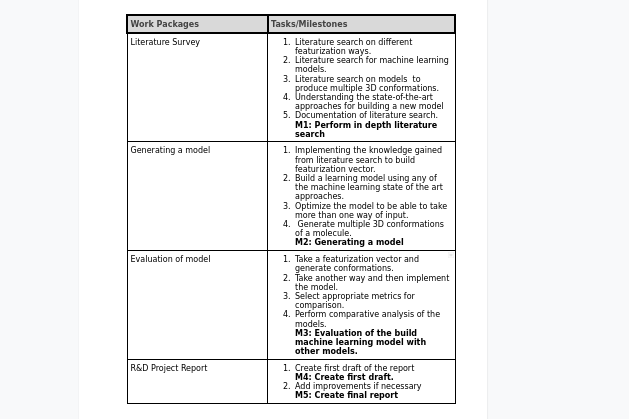
\includegraphics[width=\textwidth]{RND_reports/RND_Proposal/images/wp.png}
    \label{}
\end{figure}

\FloatBarrier


\subsection{Milestones}
\begin{enumerate}
    \item[M1] Perform in depth literature search 
    \item[M2] Implementing a model to generate 3D conformations.
    \item[M3] Evaluation of the build machine learning model with other models.
    \item[M4] First draft of R\&D report
    \item[M5] Add improvements and prepare Final R\&D report
\end{enumerate}

\subsection{Project Schedule}
See Appendix A.

\subsection{Deliverables}
\subsubsection*{Minimum Viable}

\begin{itemize}
    \item In depth literature search on different methods that are using machine learning models to generate 3D multiple conformations.
    \item Analysis of state of the art. 
\end{itemize}

\subsubsection*{Expected}
\begin{itemize}
    \item A machine learning model to generate multiple 3D conformations, based on a specific featurization vector.
    \item Comparative analysis of the generated model with state of the art models.
\end{itemize}

\subsubsection*{Desired}
\begin{itemize}
    \item Implement a model that can find similarity between molecules
   \item Model that is capable of representation learning and explainable AI.
\end{itemize}
\

\nocite{*}

\bibliographystyle{plainnat} % Use the plainnat bibliography style
\bibliography{bibliography.bib} % Use the bibliography.bib file as the source of references




\end{document}
